%======================================================================
\subsection{BW-PDM-15 --- Built, 1 Nov: project tabs, cards and pages}\label{sec:pdm15-built}
%======================================================================

\begin{figure}[!htbp]
\centering
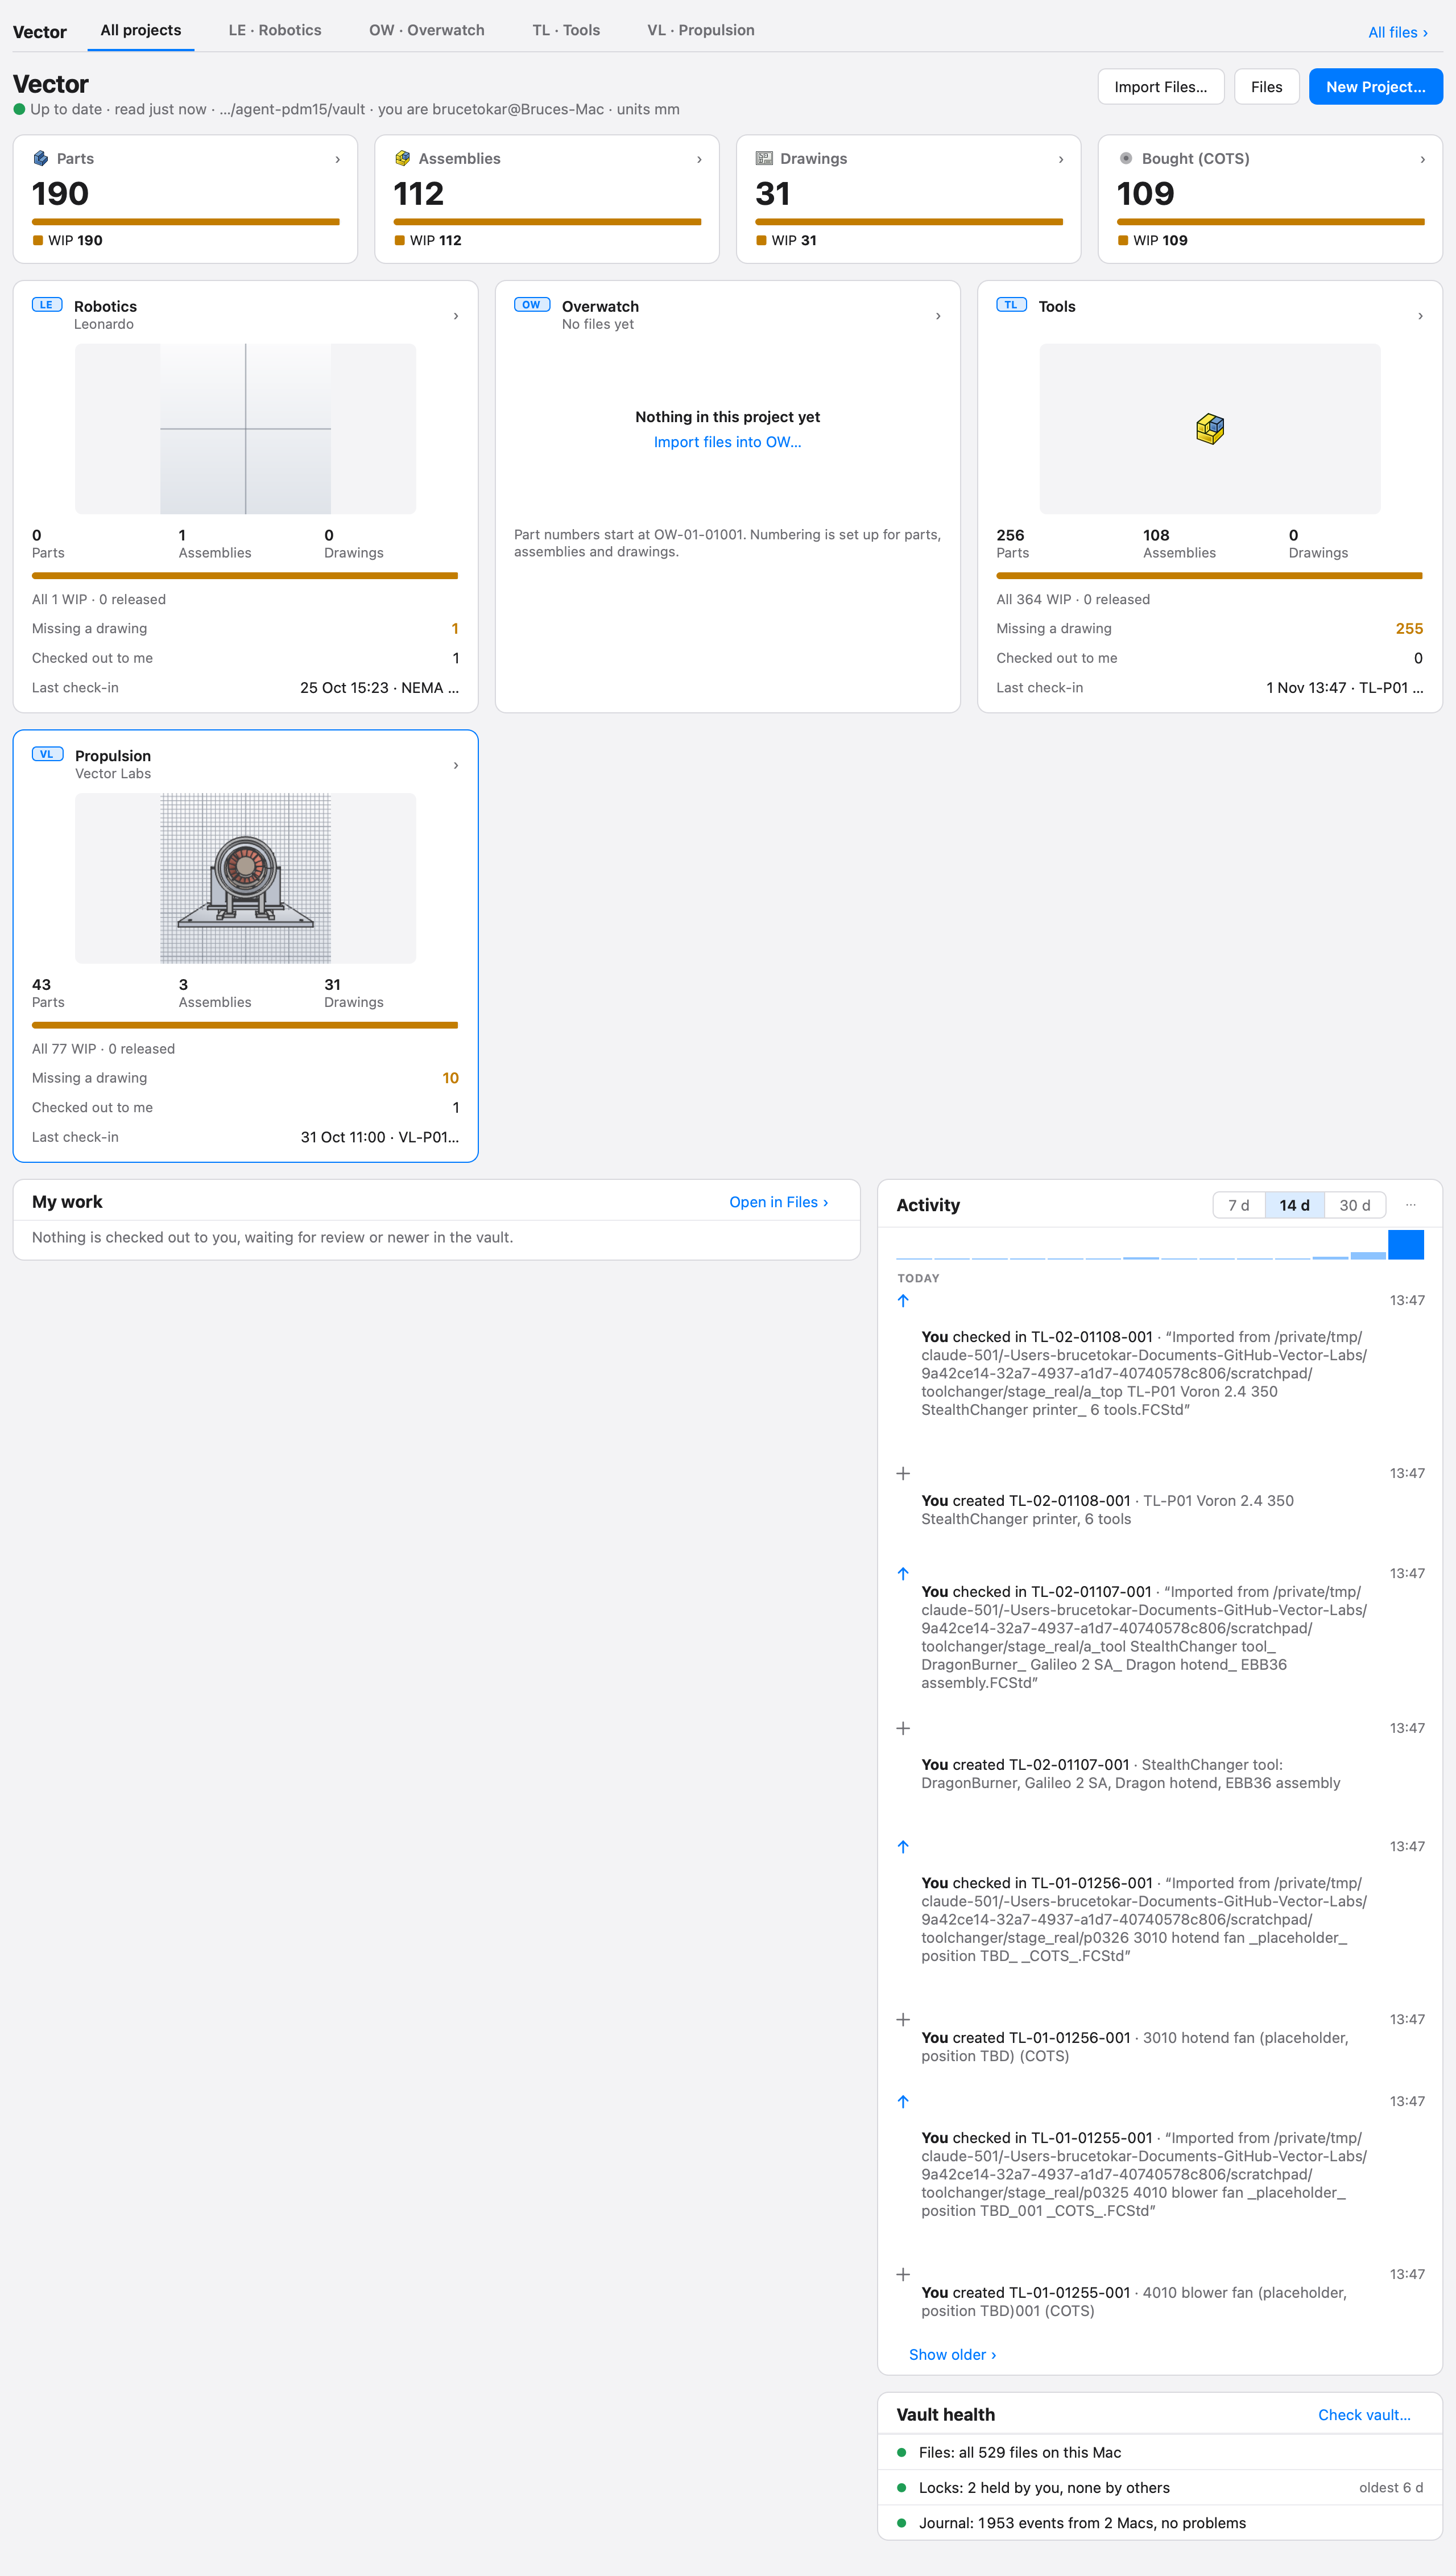
\includegraphics[width=0.95\linewidth]{fig/pdm15_all_projects.png}
\caption{All projects, on a copy of your real vault (four programs; TL is the toolchanger import): one card per project
with its top assembly's picture, counts, the WIP/released bar, files missing a drawing, checked out to you and the
last check-in; OW is the empty project's card. Activity and vault health are as before, the activity lines now name
their project. Off-screen render.}
\label{fig:pdm15-all}
\end{figure}

\begin{figure}[!htbp]
\centering
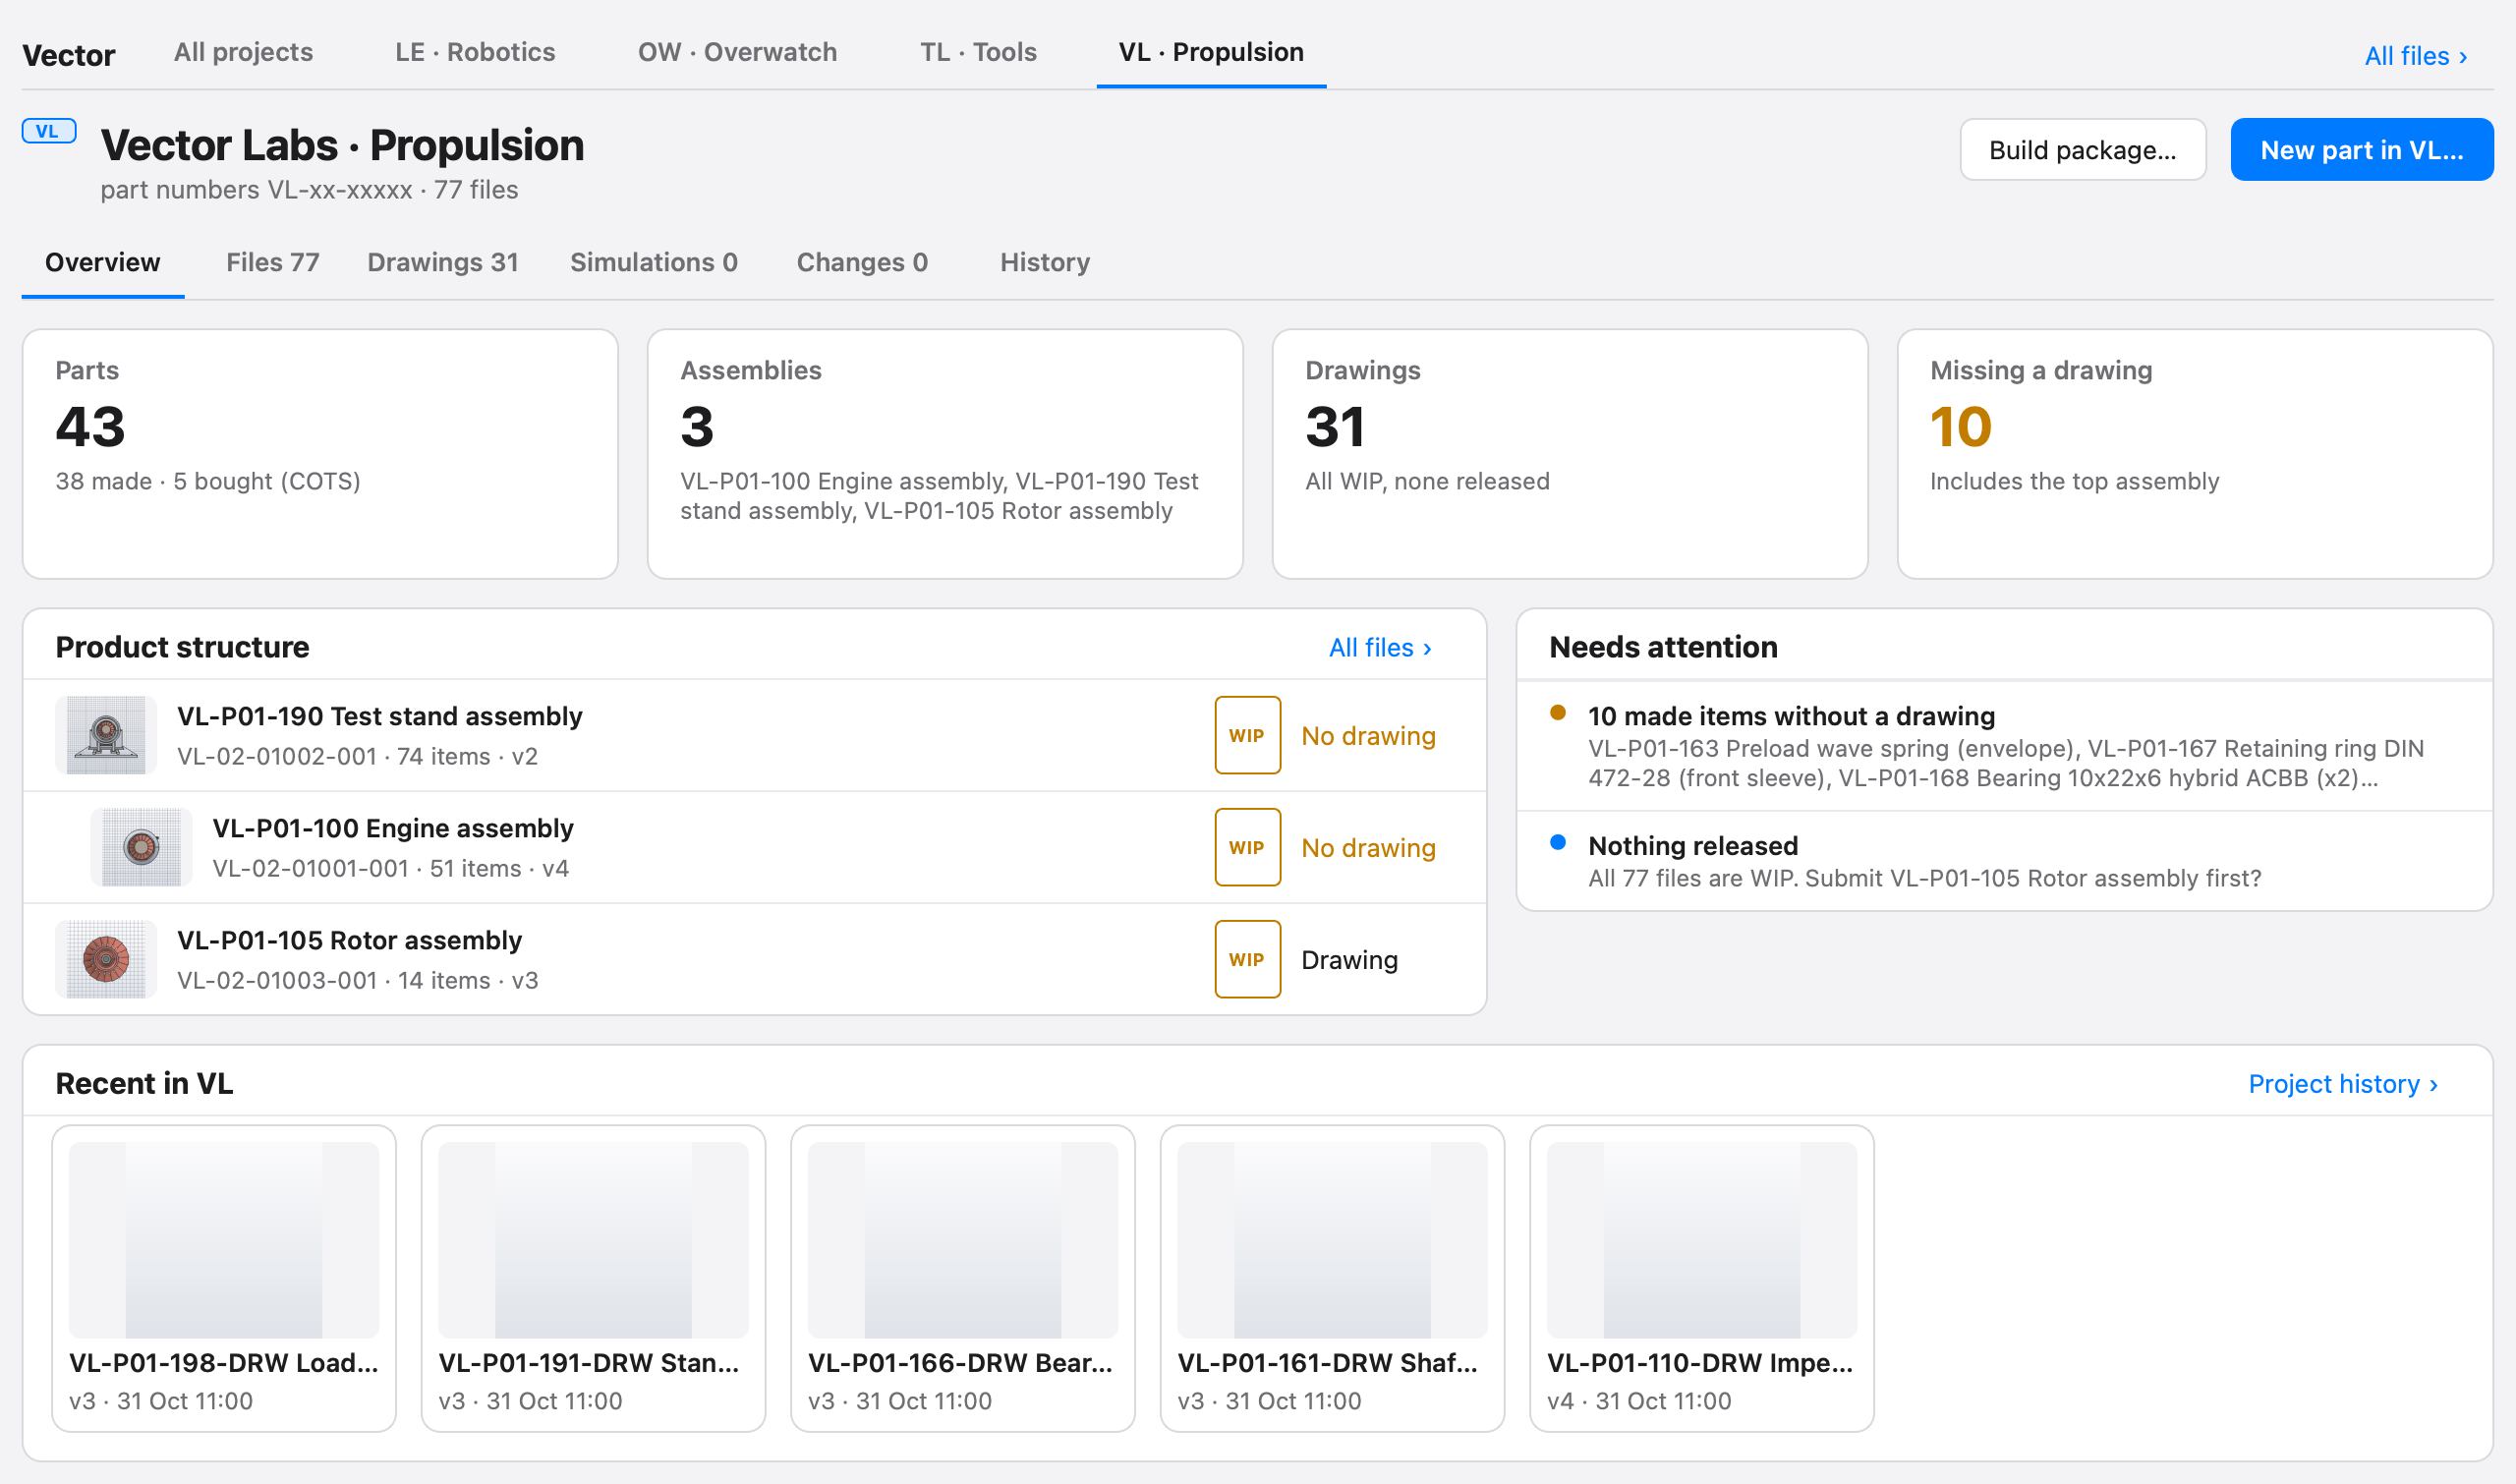
\includegraphics[width=0.95\linewidth]{fig/pdm15_project_vl.png}
\caption{The VL project page, Overview: header with \emph{Build package\ldots} and \emph{New part in VL\ldots}, tabs
with counts, the four count tiles (43 parts, 3 assemblies, 31 drawings, 10 missing a drawing, as in your mockup),
the product structure with pictures, state and drawing status, Needs attention, and recent files as picture cards.
The recent drawings show grey sheets because their saved thumbnails are blank until Refresh Pictures runs.}
\label{fig:pdm15-vl}
\end{figure}

\paragraph{What you can do now.}
\begin{itemize}[nosep]
  \item Along the top of the vault area: \emph{All projects} and a tab per project (``VL $\cdot$ Propulsion'').
        The Start page's tabs are unchanged; this strip is inside the vault dashboard.
  \item A project opens on its page: Overview, Files, Drawings, Simulations, Changes, History, each with its count.
        \emph{Files} is the PDM-13 browser moved into the page and scoped to the project (leaving the page puts it
        back on the Files tab). Count tiles, Needs attention lines and picture cards open Files filtered
        (\code{view:missing}, \code{state:wip}, a selected file). \emph{Drawings} lists the drawings with their sheets;
        \emph{Build package\ldots} runs the existing package dialog. \emph{New part in VL\ldots} is the existing New
        Part dialog with the program preselected. \emph{Changes} lists the ECRs and ECOs touching the project;
        \emph{History} is the journal's events for it.
  \item \emph{Simulations} is PDM-14's \code{vault\_trees.simulations}, scoped to the project's files. A simulation
        whose part changed is marked OUT OF DATE and adds \emph{n simulations out of date} to Needs attention.
\end{itemize}

\paragraph{Decided while building.} Pictures are read from the picture cache or the thumbnail inside the file, never by
opening a document. A project's top assembly for its card is the largest assembly no other assembly of the project
uses. A program called ``Heuretes FreeCAD - Propulsion'' shows as ``Propulsion'' with ``Heuretes FreeCAD'' under it. The old
Projects list and the type tiles stay on All projects; the cards replace the list. Files from a simulation item are
counted as files but not as parts.

\paragraph{Speed.} Everything is computed once per snapshot on the worker thread by
\file{addons/BruceWorx/bruceworx/project\_pages.py} (about 190\,kB per snapshot for the pages; assemblies' links are
cached per stored file). On a copy of your vault with 442 items and 1\,953 journal events (VL 77 files, TL 364): cold
build 150\,ms, warm 7\,ms; whole snapshot 19\,ms warm; filling the All projects view 21\,ms; opening the VL or TL page
about 90\,ms including pictures. A generated vault of 400 items builds in well under a second.

\paragraph{Tests.} Add-on: \file{test\_project\_pages.py} (14 tests: counts, structure tree, attention, recent files,
history, empty project, simulations from a fake list and with a failing API, changes, snapshot, speed) and
\file{test\_vault\_dashboard.py}. GUI: \file{TestBruceWorxProjectPage.py} (9 tests; tabs, cards, every page tab, the Files
list moving in and back, the simulation rows) with TestBruceWorxStart, VaultClient and VaultBrowser all passing.

\paragraph{Open questions.} (1) Offscreen Qt crashes this build at the 3D view, so the GUI tests and renders ran on the
normal display, windows unraised. (2) Project descriptions come from PDM-09 project records when there are any
(your vault has none). (3) Should the old type tiles go from All projects now that the cards exist?
